\documentclass[a4paper,12pt]{report}

% --- Encoding & Language ---
\usepackage[utf8]{inputenc}
\usepackage[T1]{fontenc}
\usepackage[english]{babel}

% --- Recommended for biblatex ---
\usepackage{csquotes} % <<< Wichtig für Zitate

% --- Page layout ---
\usepackage{geometry}
\geometry{a4paper, margin=2.5cm}

% --- Margin fix for todonotes ---
\setlength{\marginparwidth}{2cm} % Wichtig für todonotes
\usepackage[colorinlistoftodos]{todonotes}

% --- Graphics & Tables ---
\usepackage{graphicx}
\usepackage{caption}
\usepackage{subcaption}
\usepackage{booktabs}

% --- Math ---
\usepackage{amsmath, amssymb}
\usepackage{siunitx}

% --- Hyperlinks & references ---
\usepackage{hyperref}
\usepackage{cleveref}

% --- Bibliography ---
\usepackage[backend=biber,style=ieee]{biblatex}
\addbibresource{references.bib}

% --- Glossary ---
\usepackage[acronym]{glossaries}
%----------------  Glossary Entries  ---------------------------------------
\newglossaryentry{latex}{
    name=LaTeX,
    description={Ein Textsatzsystem für wissenschaftliche Dokumente}
}

\newglossaryentry{bfh}{
    name=BFH,
    description={Berner Fachhochschule}
}

%----------------  Acronyms  -----------------------------------------------
\newacronym{ai}{AI}{Artificial Intelligence}
\newacronym{ml}{ML}{Machine Learning}
\makeglossaries

% --- ToDo notes ---
\usepackage[colorinlistoftodos]{todonotes}

% --- Custom commands ---
\newcommand{\vect}[1]{\mathbf{#1}}
\newcommand{\TODO}[1]{\todo{#1}}

% --- Title ---
\title{Master Technical Report Template}
\author{John Doe}
\date{\today}

\begin{document}

\maketitle
\tableofcontents
\listoffigures
\listoftables
\printglossaries

% --- Chapters ---
\chapter{Introduction}
\section{Motivation}
This is the introduction. It explains the background.

\section{Goals}
The goal of this report is to provide a ready-to-use master template.

\subsection{Example Figure}
\begin{figure}[h!]
    \centering
    
\includegraphics[width=0.6\textwidth]{images/example-image.png}
    \caption{Example figure}
\end{figure}

\subsection{Glossary \& Footnotes}
Use glossary terms: \gls{ai}, \gls{ml}.  
This is a footnote example.\footnote{This is a footnote.}  
\TODO{Add more background information.}

\chapter{Methods}
\section{Experimental Setup}
The experimental setup consists of a low-pass RC filter followed by an operational amplifier (OpAmp) in an inverting configuration. The circuit was simulated and measured under varying input voltages. \cite{EinsteinCoefficientsSpringerLink}

\subsection{Circuit Design}

The test circuit used for the measurements is shown in \Cref{fig:circuit}. 
A resistor-capacitor low-pass filter was implemented to analyze the frequency response.

\begin{figure}[h!]
    \centering
    \begin{circuitikz}[scale=1.0]
        \draw
        (0,0) to[sV, l=$V_{in}$] (0,3) 
              to[R=$R$] (3,3) 
              to[C=$C$] (3,0) -- (0,0)
        (3,3) to[short, -o] (5,3) node[right]{$V_{out}$};
    \end{circuitikz}
    \caption{RC low-pass filter used for the experimental setup.}
    \label{fig:circuit}
\end{figure}

The theoretical transfer function of the RC low-pass is:
\[
H(j\omega)=\frac{V_{out}}{V_{in}} = \frac{1}{1 + j\omega RC},
\]
with cutoff frequency \(f_c = \dfrac{1}{2\pi RC}\).  
For example, using \(R=\SI{1}{\kilo\ohm}\) and \(C=\SI{160}{\nano\farad}\) yields \(f_c \approx \SI{1}{\kilo\hertz}\).

\subsection{Frequency Response}
The system was tested with sinusoidal input signals of different frequencies. The measured and simulated frequency response is shown in \cref{fig:freqresponse}.

\begin{figure}[ht]
\centering
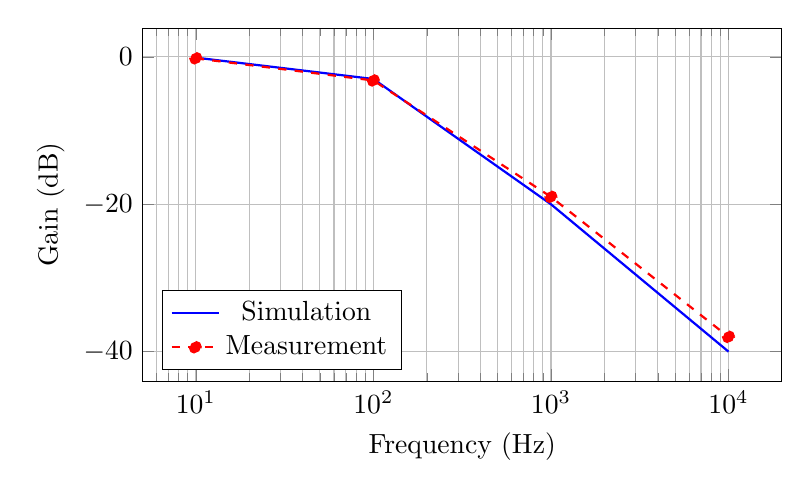
\begin{tikzpicture}
  \begin{axis}[
    width=0.8\textwidth,
    height=0.5\textwidth,
    xlabel={Frequency (Hz)},
    ylabel={Gain (dB)},
    xmode=log,
    grid=both,
    legend pos=south west
  ]
    % Simulated curve
    \addplot[color=blue, thick] table {
      10   -0.1
      100  -3
      1000 -20
      10000 -40
    };
    \addlegendentry{Simulation}

    % Measured curve
    \addplot[color=red, thick, dashed, mark=*] table {
      10   -0.2
      100  -3.2
      1000 -19
      10000 -38
    };
    \addlegendentry{Measurement}
  \end{axis}
\end{tikzpicture}
\caption{Frequency response of the circuit: simulation vs. measurement.}
\label{fig:freqresponse}
\end{figure}

\subsection{Component Distribution}
The share of components used in the experimental circuit is shown as a pie chart in \cref{fig:pie}.

\begin{figure}[ht]
\centering
\begin{tikzpicture}
  \pie[text=legend, radius=2, color={blue!50, red!50, green!50, orange!50}]{
    40/Resistors,
    30/Capacitors,
    20/OpAmp,
    10/Misc
  }
\end{tikzpicture}
\caption{Distribution of components in the circuit.}
\label{fig:pie}
\end{figure}

\subsection{Example Table}
A comparison of simulated and measured cut-off frequencies is given in \cref{tab:cutoff}.

\begin{table}[ht]
\centering
\begin{tabular}{lcc}
\toprule
 & Simulation & Measurement \\
\midrule
Cut-off frequency (Hz) & 980 & 1020 \\
Gain at 1 kHz (dB)     & -20.0 & -19.0 \\
\bottomrule
\end{tabular}
\caption{Comparison of simulated and measured results.}
\label{tab:cutoff}
\end{table}

\chapter{Results}
\section{Data Analysis}
Example formula:
\[
E = mc^2
\]

\subsection{Example Additional Figure}
Here we show an additional example image:

\begin{figure}[h!]
    \centering
    
\includegraphics[width=0.7\textwidth]{images/example-image.png}
    \caption{This is an additional example image.}
    \label{fig:example2}
\end{figure}

As shown in \cref{fig:example2}, the image demonstrates how to include graphics in LaTeX.

\section{Observations}
Discuss observations and highlight points with \TODO{Add graphs here}.

\chapter{Conclusion}
\section{Summary}
Summarize the findings and conclusions.

\section{Outlook}
Provide future work suggestions.

\printbibliography

\end{document}